%use the KomaScript styling on A4 paper
\documentclass[a4paper]{scrreprt}
%package for citing in Harvard style
\usepackage{natbib}
\bibliographystyle{agsm_paul}
\usepackage[T1]{fontenc}
\usepackage[utf8]{inputenc}
\usepackage[none]{hyphenat}
\usepackage{graphicx}
\usepackage{multirow}
\usepackage[hidelinks]{hyperref}
\usepackage{xurl}
\graphicspath{{"./figs"}}

%declare *bf* that is needed for natbib
\DeclareOldFontCommand{\bf}{\normalfont\bfseries}{\mathbf}
%set style of footnote numbering
\counterwithout{footnote}{chapter}

\begin{document}

\begin{titlepage}
\centering
{\large\textsc{Bachelor thesis}\par}
\vspace{8\baselineskip}
{\Huge The right-wing populism of the AfD party and its regional differences\par}
\vspace{2\baselineskip}
{\Large A quantitative analysis on populist antagonisms within the programmatic discourse\par}
\vspace{5\baselineskip}
{\large\textsc{submitted by\\[.5em]Dipl.-Math. Paul Keydel}\par}
\vspace{8\baselineskip}
{Freie Universität Berlin, April 2024\par}
\vfill
\raggedright
{\em 1st supervisor: Dr. Julia Reuschenbach\\}
{\em 2nd supervisor: Prof. Dr. Bruno Castanho Silva}
\end{titlepage}

\tableofcontents

%%%%%
% 1 %
%%%%%
\chapter{Introduction}
The aim of this thesis is to bla bla\\
All data files as well as all written scripts can be found on Github.\footnote{see \url{https://github.com/PaulKeydel/telegram_populism}}
%%%%%
% 2 %
%%%%%
\chapter{Populism as an ideology of democracy}
\section{What is an ideology?}
In order to understand the connection between populism and ideology, this section will outline a theoretical framework behind ideologies. There are, in general, several approaches within political theory to define or describe ideologies. For example, one might take policies into account and consider ideologies as attributions of them in a one-dimensional left-right spectrum. Such a policy-based approach can be useful for descriptive analysis of party alignment or voting behavior. \citep[p.~154]{lembcke:2014} But what is an ideology in itself?\par
The concept of attributing policies to ideologies suggests that ideologies are related to political issues and the way we think about politics. They originate from political thought, which is in turn expressed by a specific terminology and its meanings. With this, it opens up a discourse-analytical approach to ideologies that is particularly represented through the work of Michael Freeden. He claimed that the ``study of ideology becomes the study of the nature of political thought: its building blocks and the clusters of meaning with which it shapes the political worlds we populate''. \cite[p.~15]{freeden:2006} For him, the act of political thinking arises from real-world contexts and seeks interpretations of the political reality - within a specific terminological framework that is used to express and formulate these meaningful interpretations. Political thought is thus, too, a practice of building meanings and where individuals ``attempt [...] to impose specific senses on repositories of political meaning that are by their semantic nature multivalent and contestable''. \cite[p.~19]{freeden:2006} At this point, ideologies play a central role. They can structure the described process of political thought in the sense that ideologies both assign and fix specific meanings to political ideas or concepts. Freeden understands ideologies further as conceptual structures with which all political actors describe themselves, the relation between them and their relation to the surrounding world. Consequently, ideologies temporarily ``define our understanding of the political'' and they are thus dynamic, i.e. they change as political challenges of the society change. Within this dynamic alignment they also ``compete with alternative configurations over political support and over the central control of the political''. \cite[p.~14]{freeden:2006}\par
In his popular book {\em Ideologies and Political Theory} (1998) Freeden has developed a morphological approach to ideologies in order to explain and reconstruct the process of competition between conceptual elements and interpretations. His starting points are the already mentioned ``political concepts'' that stand for rather abstract ideas like ``liberty, justice, power and rights''. \cite[p.~54]{freeden:1998} These concepts are far from monolithic constructs, they rather consist of smaller {\em components} which can relate to each other and represent, through their specific configuration, the entire concept. Freeden distinguishes here between ``ineliminable'' and non-ineliminable\footnote{To be precise, non-ineliminable components are ``quasi-contingent''.} components. Ineliminable components are logically necessary, i.e. without any such components, it is impossible to derive a reasonable meaning. Thus, the set of all ineliminable components might be seen as the {\em core} of the concept, whereas non-ineliminable components ``cannot carry the concept on their own''. \cite[p.~62]{freeden:1998}\par
An analogous topology can be transferred to ideologies and conceptual structures, respectively. An ideology obtains and fixes meanings from multiple concepts and a single concept is not only determined by its components but also by its position within a greater ``idea-environment''. \cite[p.~67]{freeden:1998} In this manner, {\em adjacent concepts} emerge that, for example, share certain components and equally are part of the same ideology. Based on these considerations, Freeden postulates a three-level formation of ideologies: The most central concepts define the {\em core of the ideology}, supplemented by the concepts from the {\em adjacency} and the {\em periphery}. The example of liberalism illustrates this morphology:
\begin{quote}
    For instance, an examination of observed liberalisms might establish that liberty is situated within their core, that human rights, democracy, and equality are adjacent to liberty, and that nationalism is to be found on their periphery. \cite[p.~77]{freeden:1998}
\end{quote}
The advantage of Freeden’s morphology is that any configuration of concepts and its components is not isolated from other configurations. An ideology characterized by connections of concepts next to each other implies, inevitably, a certain ambiguity or indeterminacy, which again enables various narratives within the political struggle of consent and support. \cite[p.~155]{lembcke:2014}
\section{Populism and bridges between \guilsinglright the people\guilsinglleft\ and \guilsinglright politics\guilsinglleft}
Populism is a widely used concept, not only in political science but also in media and public discourses. There is consequently more than one theoretical embedding of populism depending on populist aspects that will be analyzed. For example, following Chantal Mouffe and Ernesto Laclau, populism can be seen as a specific discourse practice to counteract neoliberal hegemony within a post-democratic society. Their (left-wing) populism is a positively connoted strategy to re-politize society by clarifying structures of oppression and exploitation. \citep{laclaumouffe:2001} However, when it comes to how left-wing and right-wing populism can be characterized in general, other theory buildings may be taken into account.\par
According to Cas Mudde, a more general theorizing of populism rests on ideational approaches; ``conceiving it as a discourse, an ideology, or a worldview''. \cite[p.~5]{mudde:2017} Although populism can take very different shapes in terms of political intentions or communication patterns, Mudde and Rovira Kaltwasser argue that populism at its heart is a ``kind of mental map through which individuals analyze and comprehend political reality''. \cite[p.~6]{mudde:2017} This common populist feature is directly linked to Freeden's conception on ideologies since a mental map constitutes a simpler picture on politics just as an ideology ``constitutes a significant sampling from the rich, but unmanageable and partly incompatible, variety of human thinking on politics''. \cite[p.~54]{freeden:1998} But, to distinguish populism from full-developed ideologies like liberalism, Mudde and Rovira Kaltwasser suggest a {\em restricted morphology}, i.e. populist concepts cannot offer comprehensive answers to any political issue. Instead, all patterns of populism mainly appeal to {\em the people} and are limited to a facile denunciation of {\em the elite}. Mudde finally defines populism as\par
\begin{quote}
    [...] a thin-centered ideology that considers society to be ultimately separated into two homogeneous and antagonistic camps, `the pure people' versus `the corrupt elite', and which argues that politics should be an expression of the volonté générale (general will) of the people. \cite[p.~6]{mudde:2017}
\end{quote}
Aside from this antagonistic relationship between the people and the elite and its possible consequences for populist discourses, one might ask the question of what can cause populist simplifications of reality. In the light of populist tendencies in democratic systems, this question becomes even more relevant, and referring to Margaret Canovan, there are in fact inner-democratic reasons for populism. She emphasizes an essential paradox that exists in democracies: The more people participate within the political arena, the more opinions and interests are part of the democratic discourse and the more difficult it is to conceptually overlook the arena, i.e. the ``most inclusive and accessible form of politics ever achieved is also the most opaque''. \cite[p.~25]{canovan:2002} In other words, the contradiction exists between the necessity of representing the people's concerns within the political process and, individually, the impossibility of deriving clear interpretations of the entire political arena. It is hence a contradiction between ``bringing the people into politics'' and ``taking politics to the people'', and a certain part of the people respond to this by establishing populist attitudes. \cite[p.~26]{canovan:2002} Due to the complexity and variety of the political arena, people lean towards simplifications that is, the appeal to their `own' sovereignty against an unrepresentative elite that is supposed to be responsible for the lack of effective participation.\par
From a democratic point of view, the purpose of ideologies may be summed up in constructing bridges between {\em the people} and {\em politics}. They can offer a mental and intelligible map of the reality which becomes even more pressing within democracies, that are by their nature highly inclusive and complex. Populism, consequently, appears to be inherent in democracy - as the most vivid bridge. But paradoxically, according to Canovan, ideologies within democracies can always be misrepresentative regarding basic democratic principles. In this sense, the thin-centered populist ideology with its appeal to people’s sovereignty admittedly generates a simplification of the political arena but, on the other hand, creates a ``popular unity against multiplicity'' and a ``majority against minorities'', respectively. \cite[p.~26]{canovan:2002}. Such a contrariness, and in particular its discursive construction is investigated in the following section.
\section{The role of antagonisms}
Roughly speaking, antagonisms are almost always the crucial element in constructing theoretical understandings of populism regardless of whether it is left-wing or right-wing. In Mouffe's and Laclau's conception of populism as a discursive strategy, antagonisms are assumed to be the observable consequences of neoliberal hegemony. They need to be addressed by expressing all modes of oppression and exploitation equivalently in a linguistic chain associated with other social inequalities. Due to this chain of equivalent antagonisms, a discursive momentum will be established to re-politicize society and repress the neoliberal hegemony. \cite[p.~135]{laclaumouffe:2001}\par
While the antagonistic configuration of left-wing populism is based on fights against poverty, privileged classes or ecological destruction, right-wing populism usually draws on other rivalries. But, as noted in the previous section, in all cases the use of antagonisms is required for constructing a specific dichotomy of {\em the people} and {\em the elite}. Following Mudde's definition, the concepts of the people and the elite are besides {\em the general will} the core concepts forming the populist ideology. As such they divide society into two distinct groups distinguishing between ``a homogeneous {\em good} and a homogeneous {\em evil}'' \cite[p.~7]{mudde:2017}. The concept of the people is thereby rather indeterminate: Who and what are the people? One answer was given by Laclau. According to him, the constitution of the people is a performative act. Laclau argues, similarly to Freeden, that meaning emerges with and through language and especially the construction of a collective identity like the people fundamentally depends on articulations between a logic of difference and a logic of equivalence. \cite[p.~x]{laclau:2005} Regarding the `good versus evil' dichotomy, he notes the importance of differential articulations within the production of meaning:
\begin{quote}
    This division [of society] presupposes the presence of some privileged signifiers which condense in themselves the signification of a whole antagonistic camp (the 'regime', the 'oligarchy', the 'dominant groups', and so on, for the enemy; the 'people', the 'nation', the 'silent majority', and so on, for the oppressed underdog - these signifiers acquire this articulating role according, obviously, to a contextual history). \cite[p.~87]{laclau:2005}
\end{quote}
From this perspective, it becomes obvious how antagonistic articulations meaningfully fill the political concept of the people that initially is just an ``empty signifier''. \cite[p.~72]{laclau:2005} Populism of all political colors hence requires several kinds of antagonisms to constitute the opposition between {\em us} and {\em them}. On the other side, several equivalent articulations are the discursive basis for the {\em common cause}, i.e. they (re-)produce a ``shared identity'' between different groups and generate (political) affiliation. \cite[p.~9]{mudde:2017}\par
Putting all of this together, we can now identify the antagonistic nature of populism as an ideology of democracy. As the previous section pointed out, the people and the elite are supposed to be separated along the gap of power and the lack of effective participation. This specific dichotomy is not only articulated by attacks against selfish politicians, corrupt bureaucrats or democratic institutions in themselves, but also by attacks against those who are being identified as clients of the elite. That can involve asylum-seekers, migrants and certain minority groups and, typically, these groups are being negatively framed as ``beneficiaries of taxes paid by ordinary, hard-working people''. \cite[p.~32]{canovan:2002} This shows very plainly that racist discourses from the right-wing spectrum might affect the antagonistic articulation even more due to inherent practices of social othering. In general, since political concepts of right-wing movements or parties are related to multiple adjacent ideologies like nativism, authoritarianism or even Nazism, pure populist discourses can partly merge with others. Consequently, if one analyzes right-wing populism as we will do in the next chapter, the antagonistic constitution of {\em the people} should be considered multi-dimensionally.
%%%%%
% 3 %
%%%%%
\chapter{The AfD party and its right-wing populism}
\section{The party between populism and right-wing ideologies}
Within the political landscape in Germany, the AfD party ({\em Alternative für Deutschland}) became gradually successful and concerning current surveys they were the second political force in February 2024.\footnote{see \url{https://www.zdf.de/nachrichten/politik/politbarometer-afd-bsw-schuldenbremse-rechtsextremismus-ukraine-100.html}} The AfD party was founded in 2013 and can be seen as a so-called challenger party that claims to break with the established mainstream and the `old' tradition of catch-all parties. \citep{devries:2020} Nevertheless, the success of the AfD party is not merely a German phenomenon. Particularly the populist and right-wing challenger parties in Europe have been rising since the 1980s when one considers, for example, the French {\em Rassemblement national}, the Belgian {\em Vlaams Belang} or the Italian {\em Lega}. \cite[p.~30]{devries:2020} All these parties have a strong appeal to {\em the people} in common, and also they share other ideological key elements like xenophobia or nativism. That is because populism as a thin-centered ideology of democracy is a malleable conceptual structure and ``can easily be integrated into another more complex host ideology''. \cite[p.~19]{devries:2020}\par
In the book {\em The Far Right Today} Cas Mudde describes such interrelated ideologies that might serve as a host ideology. Following Mudde, the far right is first of all split into two groups, the ``extreme right'' and the ``populist radical right''. While the first group ideologically builds on historical fascism and fundamentally rejects democracy, the populist radical right supports democracy to some extent. Their ideological core consists of populism, nativism (a combination of both nationalism and xenophobia) and authoritarianism. \cite[p.~24]{mudde:2019} These three concepts generate a broader ideology according to which, first, society must be strictly ordered, second, citizenship is based on ethnicity and, third, mainstream parties keep the people from power. The consequent host ideology can additionally contain certain anti-religious elements such as antisemitism which has been part of right-wing ideologies since the twentieth century. \cite[p.~28]{mudde:2019} However, the ideological manifestation of far-right parties changes over time and a party's shift from a populist radical right ideology to extreme right might be fluent.\par
Especially the AfD party, in terms of its ideological basis, has been subject to change since its foundation. The party initially was a eurosceptic and economically liberal project but changed fast to a right-wing project during the migration crisis in 2014: According to their political communication on Facebook between 2013 and 2017, Arzheimer and Berning showed that the party ``has developed a clear focus on common populist radical right topics''. \cite[p.~3]{arzheimer:2019} But, even though the AfD party can be identified as a populist radical right project, extremist or conspiratorial tendencies might have increased the ideological setting in the last years, possibly due to the Corona pandemic or other crises affecting the ordinary people's lives. Indeed, other research on partisan social media communication indicated that Facebook posts of the AfD party are, among populist elements, significantly crisis-related. \citep{gruendl:2022} Populist radical right communication generally embeds such narratives to emphasize that the government has failed or to reify the repression of the people through misguided elitist policies.\par
Taking this into account, it becomes clear that the ideology of far-right parties has a multidimensional nature. The ideological core can admittedly be reduced to a few prominent concepts but all these concepts in turn reveal a variety of communicational patterns. The antagonistic logic of their ideological communication links to different concepts within the given socio-political preconditions. Regarding the AfD party, the question arises of how ideological elements and the corresponding antagonistic patterns possibly have changed. In other words, did the AfD party create a homogeneous radical right populism or is their (host) ideology region-dependently configured? The following sections and mainly the next chapter will attempt to answer this question based on AfD manifestos for the federal state elections.
\section{Ideological antagonisms and discursive differences between federal states}
Like almost all German parties, the populist radical right AfD party is organized in state associations (``Landesverbände''), i.e. the party is independently represented in each of the 16 federal states in Germany. And, because ideologically induced antagonisms and prejudices can both regionally and temporally be produced, the level of the federal states is a helpful framework to identify possible differences. On this state's level, one can further argue that there are at least two strong indicators for a non-homogeneous radical right populism of the AfD party. First, between 2021 and 2023 the German national intelligence service {\em Verfassungsschutz} categorized the AfD party in three federal states (Thuringia, Saxony and Saxony-Anhalt) as anti-constitutional and right-wing extremist.\footnote{see \url{https://www.tagesschau.de/inland/innenpolitik/verfassungsschutz-afd-sachsen-rechtsextremistisch-100.html}} This clearly shows that mainly East-German AfD state associations above average tend to extremist positions which is also assumed by some political theorists. For example, Pfahl-Traughber argues that the party's extremist wing (called ``der Flügel'' and concentrated around the powerful leader {\em Björn Höcke}) is with a view to party conferences less dominant in West Germany. \cite[p.~37]{pfahl:2019} Thus, for the study of ideological heterogeneity, the federal states seem to be appropriate units of analysis and in terms of the antagonistic constitution of {\em the people} we should most likely expect differences between East and West Germany.\par
To figure out these differences one might again take social media communication into account. In the following, I want to present an approach using party-owned and public Telegram channels from different AfD state associations. All these regional channels serve as a news service, i.e. messages only come from the AfD party. The data consists of a total of 1138 messages scraped between November 2023 and February 2024 from the country-wide channel of the party and from 8 channels on state-level: Thuringia, Saxony, Brandenburg, Bavaria, North Rhine-Westphalia, Rhineland-Palatinate, Saarland and Schleswig-Holstein. The analysis of the collected messages leads to two findings: First, many messages are just internal announcements and contain barely anything about ideological positions. Second, the political content of all other messages is surprisingly very similar, no matter what region is being considered. The majority of those messages refer to everyday news but the language itself is rather simple and regionally unspecified. As a consequence, a short-run analysis of the party's official Telegram communication is not the approach of choice if one is interested in ideological differences. Nevertheless, the data is helpful to get at least a first impression of relevant antagonisms that are used within the discourse. For this purpose, one can consider only messages that have received feedback from channel members (feedback means to assign an emoji to a message) in order to get rid of irrelevant messages. Then, within the remaining messages, we look for the most frequent words and illustrate them as a word cloud, the larger the font size the more frequent the word. (see Fig. \ref{fig:fig1}). It turns out that the Telegram communication clearly shows a set of nativist and populist keywords. For example, keywords like {\em Remigration, Migranten, Deutschland} are signifiers for a nationalist and nativist worldview, whereas words like {\em Altparteien, Ampel-Regierung, Volk, Bauern} indicate the populist dimension.\par
\begin{figure}[ht]
    \centering
    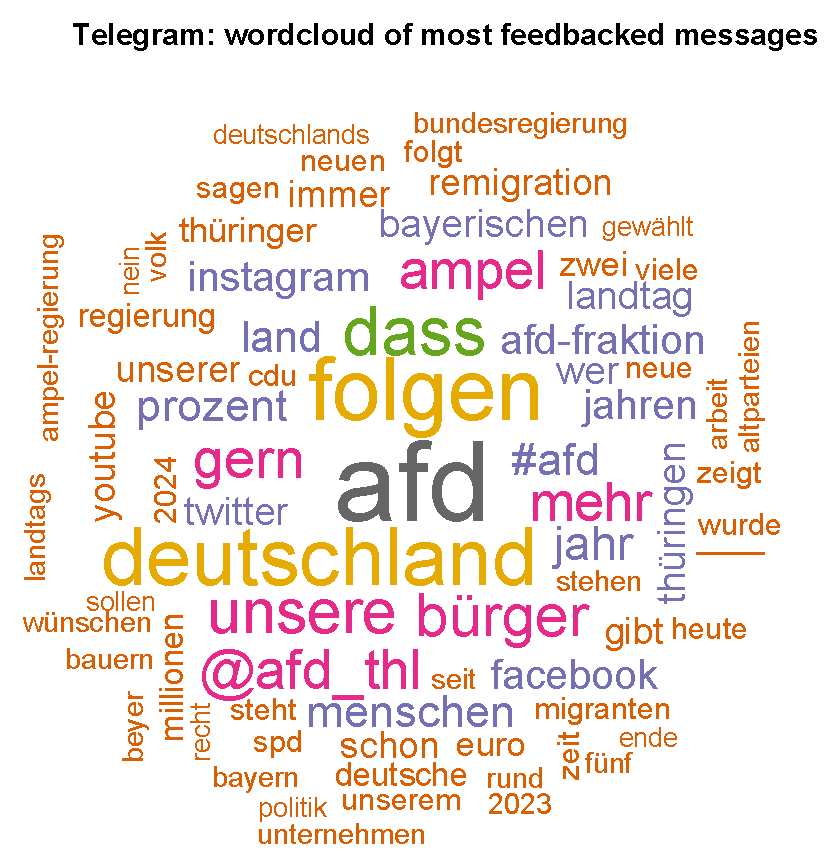
\includegraphics[width=0.6\textwidth]{telegram_wc_most_feedbacked-crop.pdf}
    \caption{Recent communication on Telegram}
    \label{fig:fig1}
\end{figure}
To sum up, the Telegram analysis in part is coincident with our theory. The AfD party as a far-right project truly uses antagonistic language against the government and immigration and, thus, confirms the assumption of both a nativist and a populist core. But what else do we learn from the above approach? Especially because we could not find reliable differences between the federal states we should consider the spatial dimension more closely. The absence of spatial differences might be traced back to the fact that there are just no differences. Even though political researchers widely agree with the ideological heterogeneity of the party, the differences might be less obvious and more subtle - ideological heterogeneity does not necessarily have to find expression in communication on Telegram. Instead, one should rather take a deep dive into the manifestos of the party. They typically offer more information in terms of the actual ideological orientation. \cite[p.~7]{pfahl:2019} That is because manifestos have their origins in a democratic party-internal process, i.e. they are the `intellectual property' of the entire party and in this sense, they represent more than a single social media team. Many other research projects in the field of party comparisons are thus based on manifestos, for example, if one is interested in populist far-right framings across European countries. \citep{kranert:2019} The antagonism analysis of this thesis is intended to follow such approaches, i.e. we put Telegram aside and will instead focus on AfD manifestos.\par
In addition to the spatial dimension, we should finally consider the temporal dimension. The Telegram analysis with its restricted timescale neglects temporal aspects almost completely although, in historical terms, political thought, ideology and democracy continuously changed over time. Compared to the spatial dimension, it is probably the most relevant axis and we should include this axis not least because it allows us to analyze regional differences time-dependently. In this context, we immediately derive a benefit from the manifestos because they already contain the time dimension. As periodic and programmatic pictures they might help us to comprehend the ideological (re-)positionings of the AfD party. Putting all this together, I propose an analysis based on the last two federal state elections and the associated AfD manifestos which allows us to consider ten years of the party's history in each federal state.
\section{Towards an analysis of the party manifestos}
On the journey towards an analysis of the AfD manifestos at the level of the federal states, there is one last open question: How can one measure ideological antagonisms? This thesis first of all proposes a quantitative research design based on so-called dictionaries. As the term suggests it is a predefined list of words to a specific category. Within the textual data, the occurrence of all those words is then counted to see how significant the corresponding category is. Such a dictionary-based analysis can easily be implemented in software and is widely used as an alternative to qualitative content analysis.\par
For demonstration purposes, this section first refers to an approach from Rooduijn and Pauwels measuring populism by use of a relatively simple dictionary. \citep{rooduijn:2011} With a manually coded dictionary, they compare the quantity of populist keywords between both left-wing and right-wing parties from the United Kingdom, the Netherlands, Germany and Italy. Although the dictionary only consists of a few stems they achieve good results. Their performed cross-check with a classical content analysis shows that the dictionary-based approach can measure populism between cases and over time only slightly more inexact than the qualitative method. The mismatch of accuracy is most likely reducible to the underdetermination of the manually generated dictionary. \cite[p.~1279]{rooduijn:2011}\par
It becomes clear that the terminological composition of the dictionary is the crucial factor in obtaining reliable measurements. Thus, modern dictionaries are increasingly being trained using computerized and statistical methods. The underlying idea behind this is to progressively add contextual words to the dictionary starting from a manually collected set of conclusive keywords. For example, one can build an iterative refinement of the dictionary based on neighboring words: that is, add all those words occurring most frequently within the sentences that contain keywords from the previous iteration. Alternatively, the iterative refinement can be done manually by adding optional words that effectively enhance the dictionary performance.\par
For the analysis of the AfD manifestos, fortunately, we can draw on such an iteratively generated dictionary constructed by Cornelius Puschmann. \citep{puschmann:2022} The so-called {\em RPC-Lex} (RPC stands for right-wing populist and conspiracy discourse) was trained on a wide range of textual data including, among others, central books and media of the German far-right movement: {\em The Protocols of the Elders of Zion}, Compact-Magazin, KenFM, Alex Jones, Daniele Ganser, Eva Herman. \cite[p.~1153]{puschmann:2022} Moreover, the authors generated three main categories to detect different aspects of the German right-wing conspiracy discourse, i.e. the {\em RPC-Lex} was designed for analyzing either language style (e.g. the degree of manipulation and scandalization), topoi (e.g. nationalism, protest, conspiracy) or antagonisms. In sum the {\em RPC-Lex} contains 13 sub-dictionaries, in particular four sub-dictionaries related to ideological far-right antagonisms: anti-elitism, anti-immigration, antisemitism and anti-gender. These four sub-dictionaries were additionally tuned by using (a) terms referring to specific political actors, (b) terms from various explorative web searches (websites like {\em WikiMANNia} and {\em Metapedia}), and (c) terms from relevant literature. \cite[p.~1154/55]{puschmann:2022} At the end the authors validated all sub-dictionaries by comparing the classification results both to other German-language dictionaries and to judgments of human coders.
%%%%%
% 4 %
%%%%%
\chapter{An analysis of antagonisms within AfD manifestos}
\section{A dictionary-based approach with \em RPC-Lex}
This chapter is going to demonstrate a possible empirical approach to examine regional differences between dichotomous {\em us} versus {\em them} constructions within the 16 AfD state associations. The central points are the generated narratives of enmity within the party‘s programmatic discourse from which we can infer a different ideological positioning. According to evaluations of scientists and journalists, it is most likely the influence of the party-internal extremist wing that might be responsible for regionally dependent differences and, under that assumption, the antagonistic articulation should differ mainly in the usage of racist and anti-immigration terms.\par
The analysis is in sum based on 30 manifestos from the last and second last state elections, i.e. the data corpus covers the programmatic development of the AfD party from 2014 to 2023. A precise overview of available AfD manifestos can be found in table \ref{tab:tab1}. All listed manifestos were either taken from official party websites or from the nonpartisan organization {\em Abgeordnetenwatch}. In preparation for the proposed content analysis, the manifestos had to be converted from pdf file format to plain text which was realized by employing the {\em PyPDF2} library for Python. The resulting text corpus was then analyzed in terms of far-right antagonisms given by the {\em RPC-Lex} dictionary from Puschmann et al. As the previous section already pointed out, the authors developed four sub-dictionaries that can detect anti-elite, anti-immigrant/islamophobic, anti-gender and antisemitic language. We have also pointed out that especially the antagonisms against the elite, the immigrants and the Jewish community are the main enmities of populist far-right parties and potential ideology-induced language differences should primarily be revealed within these three categories. Nonetheless, we additionally included the anti-gender category in the analysis because far-right parties quite often return to traditional gender role models and express their resentments towards feminist and socially progressive movements. In this sense, feminist models of gender and family are just as little part of {\em the people}.\par
On the technical side, the quantitative analysis is mainly built on the {\em quanteda} package for R, offering various functionalities for managing and analyzing text. \citep{quanteda} Furthermore, the {\em quanteda} package provides a simple framework for handling and applying dictionaries. It counts the number of keyword matches and calculates relative shares of each dictionary category, respectively.
\begin{table}\begin{center}
\caption{Available (X) AfD manifestos}
\label{tab:tab1}
\begin{tabular}{c c c c}
    \hline
    state & region & second last election & last election \\ [0.5ex]
    \hline\hline
    \multirow{2}{*}{Baden-Württemberg [BW]} & \multirow{2}{*}{West} & 2016 & 2021 \\ && (X) & (X) \\
    \hline
    \multirow{2}{*}{Bavaria [BY]} & \multirow{2}{*}{West} & 2018 & 2023 \\ && (X) & (X) \\
    \hline
    \multirow{2}{*}{Berlin [BE]} & \multirow{2}{*}{Berlin} & 2016 & 2021 \\ && (X) & (X) \\
    \hline
    \multirow{2}{*}{Brandenburg [BB]} & \multirow{2}{*}{East} & 2014 & 2019 \\ && (X) & (X) \\
    \hline
    \multirow{2}{*}{Bremen [HB]} & \multirow{2}{*}{West} & 2018 & 2023 \\ && (X) & (X) \\
    \hline
    \multirow{2}{*}{Hamburg [HH]} & \multirow{2}{*}{West} & 2015 & 2020 \\ && (X) & (X) \\
    \hline
    \multirow{2}{*}{Hesse [HE]} & \multirow{2}{*}{West} & 2018 & 2023 \\ && (X) & (X) \\
    \hline
    \multirow{2}{*}{Mecklenburg-Vorpommern [MV]} & \multirow{2}{*}{East} & 2016 & 2021 \\ && (X) & (X) \\
    \hline
    \multirow{2}{*}{Lower Saxony [NI]} & \multirow{2}{*}{West} & 2017 & 2022 \\ && (X) & (X) \\
    \hline
    \multirow{2}{*}{North Rhine-Westphalia [NRW]} & \multirow{2}{*}{West} & 2017 & 2022 \\ && (X) & (X) \\
    \hline
    \multirow{2}{*}{Rhineland-Palatinate [RLP]} & \multirow{2}{*}{West} & 2016 & 2021 \\ && (-) & (X) \\
    \hline
    \multirow{2}{*}{Saarland [SL]} & \multirow{2}{*}{West} & 2017 & 2022 \\ && (-) & (X) \\
    \hline
    \multirow{2}{*}{Saxony [SN]} & \multirow{2}{*}{East} & 2014 & 2019 \\ && (X) & (X) \\
    \hline
    \multirow{2}{*}{Saxony-Anhalt [ST]} & \multirow{2}{*}{East} & 2016 & 2021 \\ && (X) & (X) \\
    \hline
    \multirow{2}{*}{Schleswig-Holstein [SH]} & \multirow{2}{*}{West} & 2017 & 2022 \\ && (X) & (X) \\
    \hline
    \multirow{2}{*}{Thuringia [TH]} & \multirow{2}{*}{East} & 2014 & 2019 \\ && (X) & (X) \\
    \hline
\end{tabular}\end{center}\end{table}
\section{Results for the last two state elections}
Once all preprocessing steps are done it is possible to apply the {\em RPC-Lex} to the corpus consisting of all available AfD manifestos. Since the dictionary is grouped into three main categories (antagonisms, language style and topoi), we can initially analyze the corpus from that general perspective. As figure \ref{fig:fig2} shows, antagonistic content only represents approximately one-ninth of the whole programmatic discourse. The biggest amount of words within the corpus, approximately two-thirds, could not be classified by the {\em RPC-Lex}. However, this is not surprising. An arbitrary text corpus generally contains thousands of different words: stopwords, insignificant adjectives or verbs, numbers, hyperlinks, etc. On the other side, the sub-dictionaries for anti-immigrant and anti-elite language contain only about 1500 words each, the other two sub-dictionaries for both anti-gender and antisemitic language even less. But it is still an interesting result that all three main categories have approximately the same number of matching words.\par
\begin{figure}[ht]
    \centering
    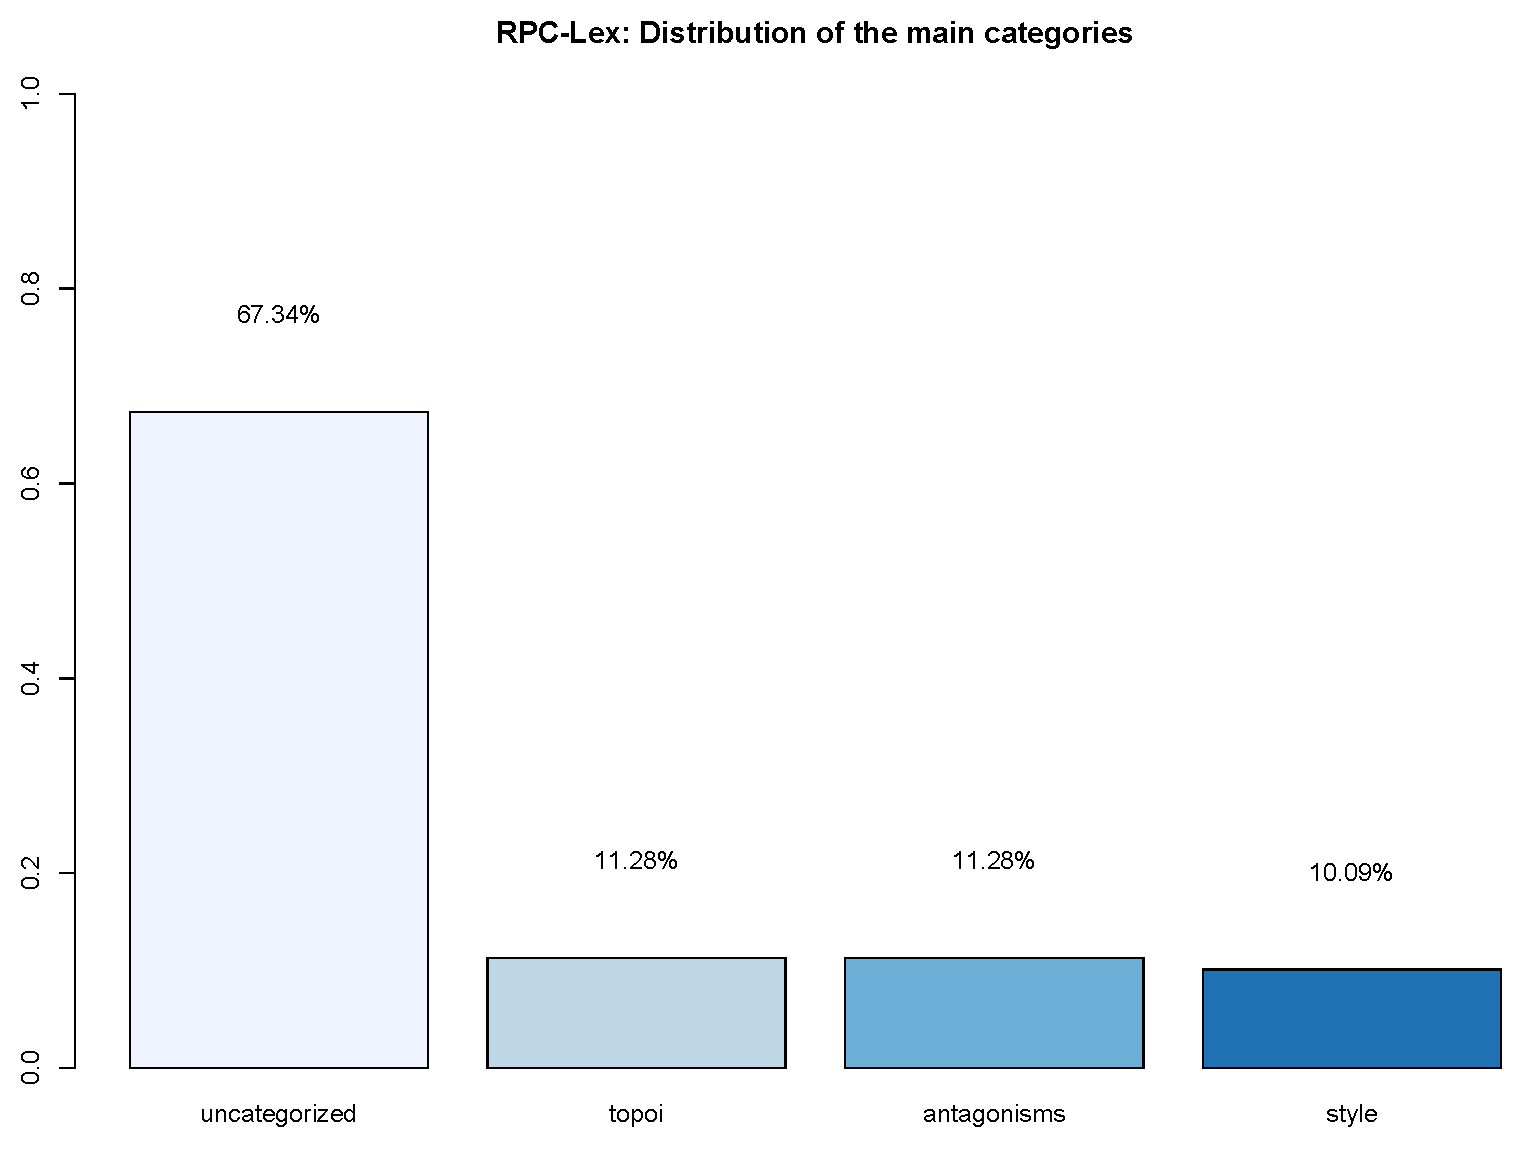
\includegraphics[width=0.7\textwidth]{manifestos_grouped_dict-crop.pdf}
    \caption{Relative shares of main categories within the entire corpus}
    \label{fig:fig2}
\end{figure}
We now want to restrict ourselves to pure antagonistic language. The goal is to split the corpus into both election periods and determine the distribution of the four ideology-related antagonisms within each period. According to table \ref{tab:tab1}, the first period ranges from 2014 to 2018 and the second period from 2019 to 2023. It is important to note that we ensure comparability between both periods, i.e. we need to normalize the distribution of the sub-dictionaries in each federal state. That means nothing else than requiring that the relative shares of the four sub-dictionaries in sum equals 1 in each federal state. The results are presented in figure \ref{fig:fig3} and \ref{fig:fig4}.\par
\begin{figure}[ht]
    \centering
    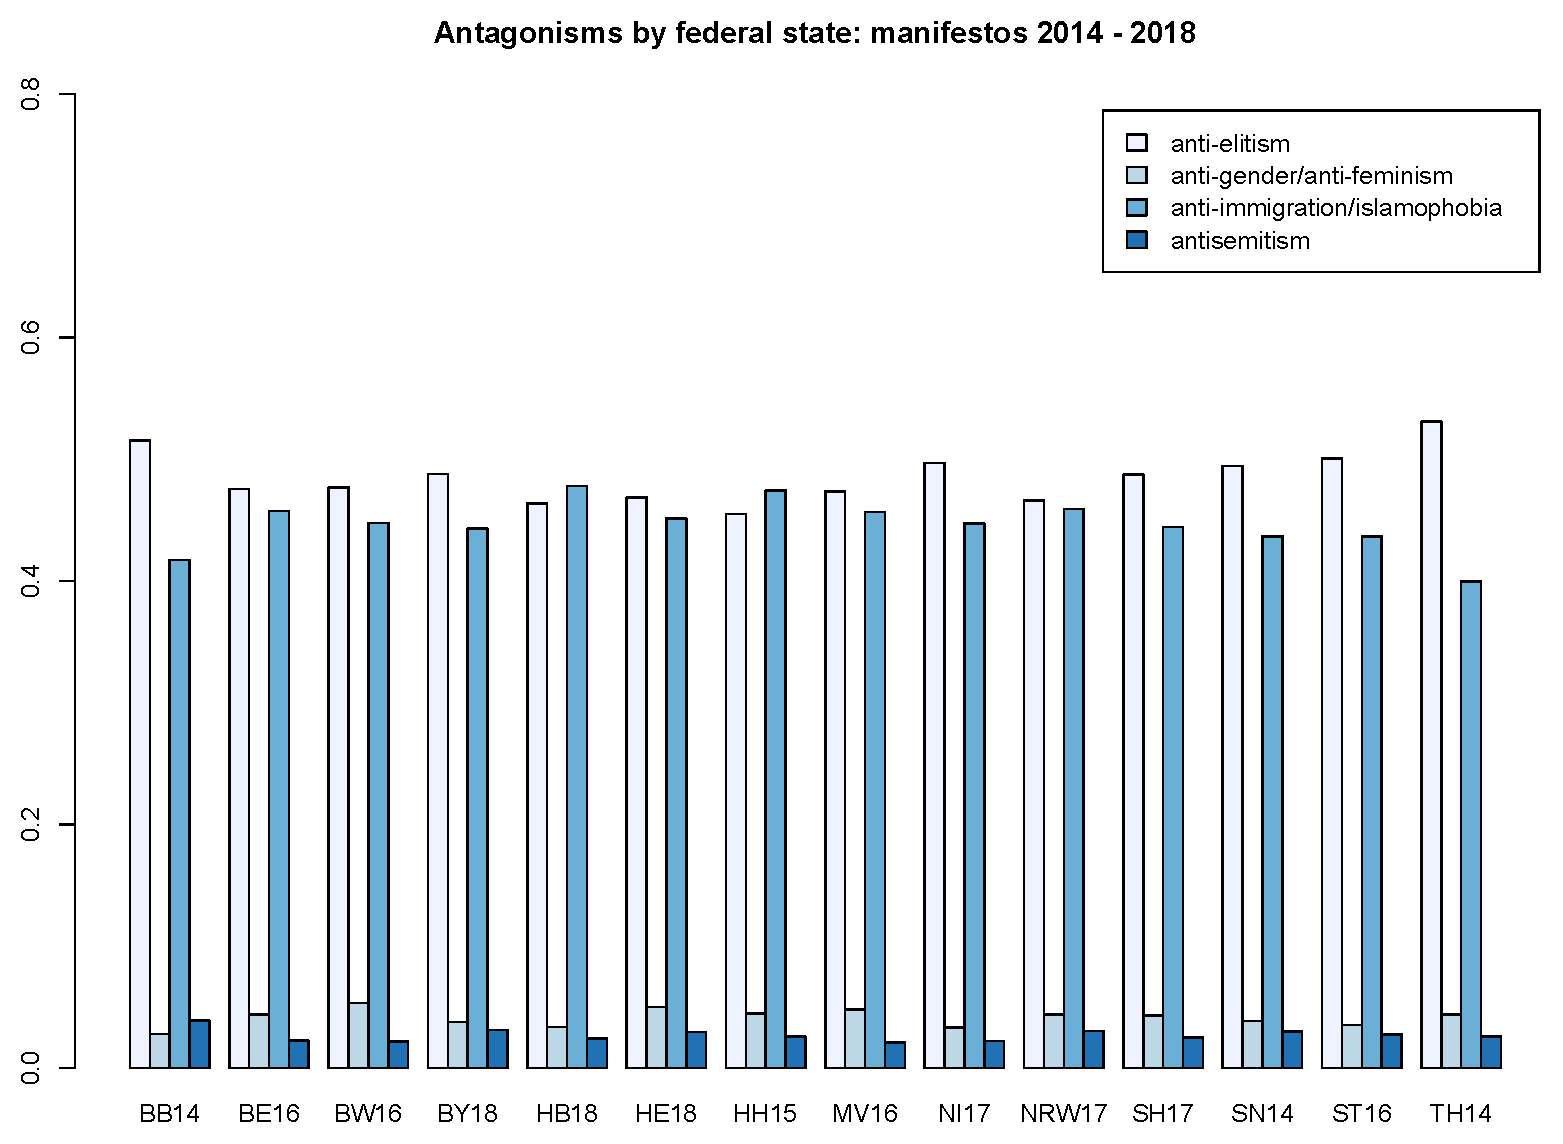
\includegraphics[width=\textwidth]{manifestos_dict_states_2013-crop.pdf}
    \caption{Relative shares of antagonism categories from 2014 to 2018}
    \label{fig:fig3}
\end{figure}
\begin{figure}[ht]
    \centering
    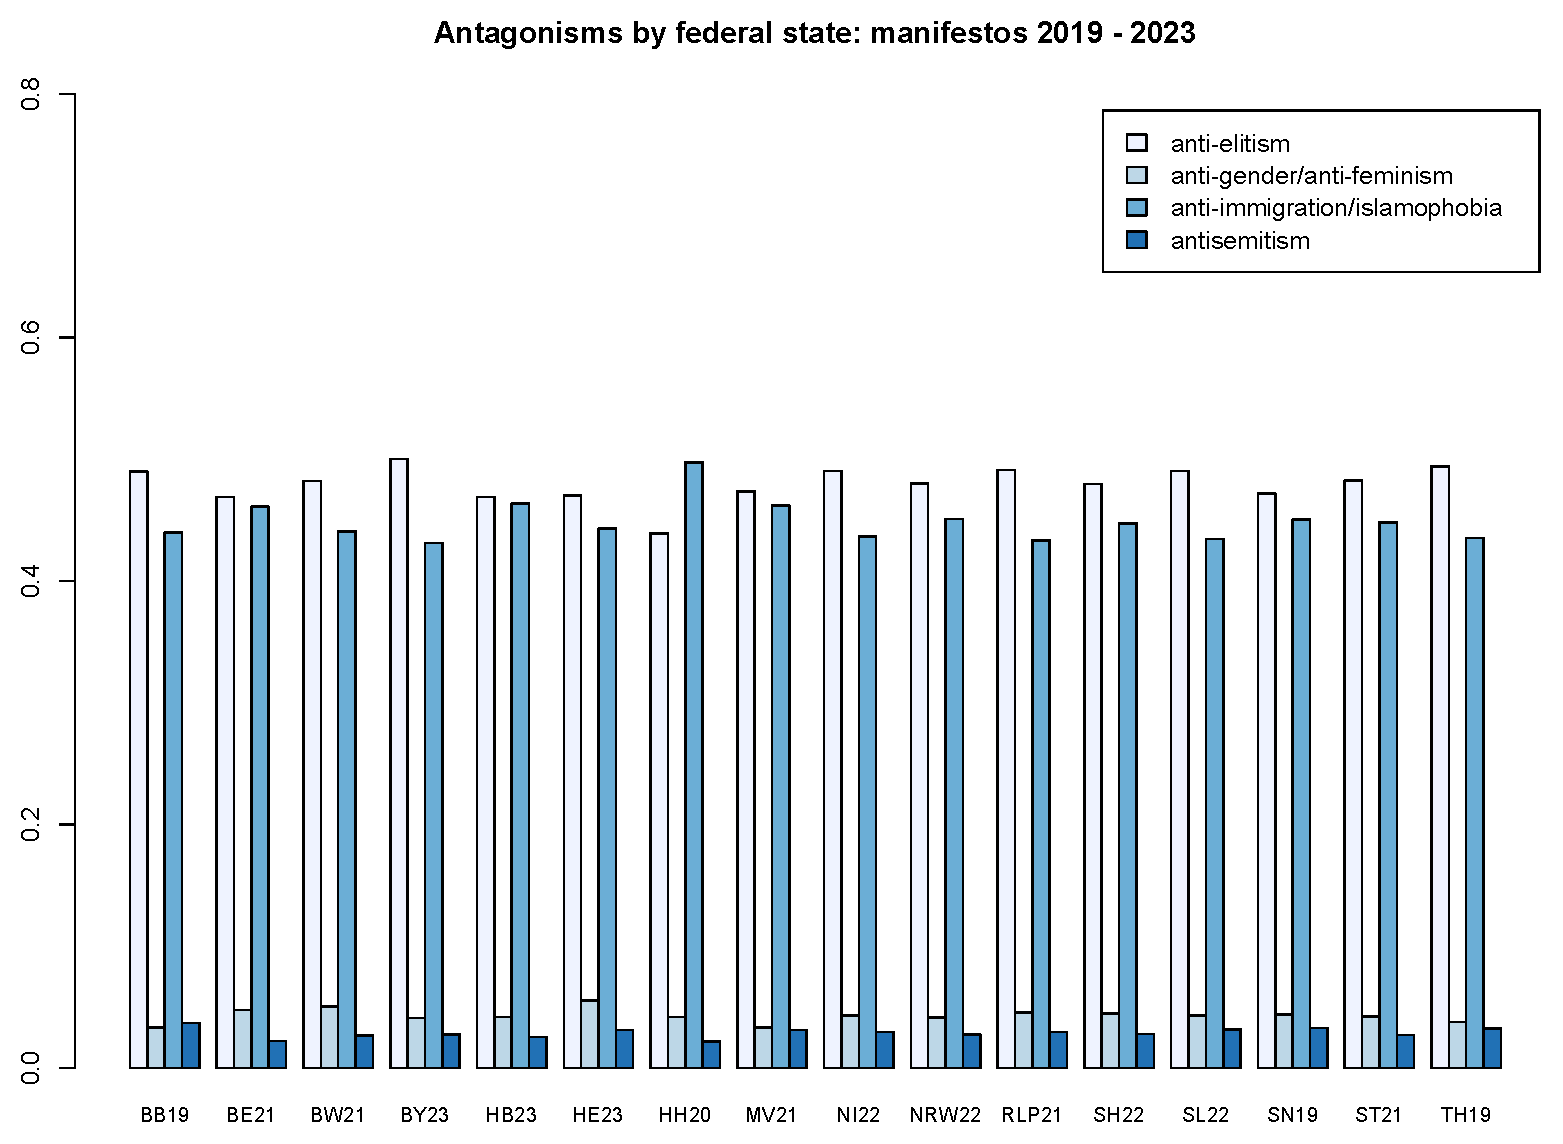
\includegraphics[width=\textwidth]{manifestos_dict_states_2018-crop.pdf}
    \caption{Relative shares of antagonism categories from 2019 to 2023}
    \label{fig:fig4}
\end{figure}
Both figures clearly show a dominance of an antagonistic articulation against the elite and immigrants regardless of time and region, which is also in line with the party's communication on Telegram investigated earlier. Almost all manifestos within the corpus are primarily characterized by an anti-elitist language, followed by a strong influence of anti-immigrant language. In combination, both kinds of antagonisms affect over 80\% of the programmatic discourse whereas anti-gender attitudes and mainly antisemitism play a rather marginal role. This repetitive pattern clarifies that the AfD party has been a populist far-right party from its beginning. And even though there might have been developments in a more extremist direction, the data can show that racist enmities have always been one of the ideological core elements besides the strong appeal to {\em the people}. In other words, social othering and narratives against democratic institutions are two integral parts of separating {\em them} from {\em us}. However, considering each single election period, regional differences in themselves are hard to identify because the distributions are just too similar. Even between East and West Germany, there are no obvious differences except that the AfD party in West German city-states has sometimes more prejudices against immigrants than against the elite (Bremen and Hamburg). All in all, one barely finds generalizable differences by looking separately at the two election periods and it is maybe more convincing to consider the temporal changes which we will do in the next section.
\section{Temporal changes between East and West Germany}
As mentioned before, both election periods allow us to take the time dimension into account and a full observation of the party‘s history becomes possible. Due to the continuous change of political thought and political discourses, we can be hopeful to see more regional differences if one compares the manifestos temporally, with a five-year distance according to the election rules in the federal states: How has a single AfD state association changed its ideological prejudices within one legislative period? Referring back to the results of the previous section, the change of antagonistic discourses can simply be calculated by subtracting the relative shares of a specific antagonism between the two moments in time. The development from the oldest manifesto to the newest is shown in Figure 4.4 (note that Rhineland-Palatinate and Saarland had to be excluded due to the missing manifestos).\par
\begin{figure}[ht]
    \centering
    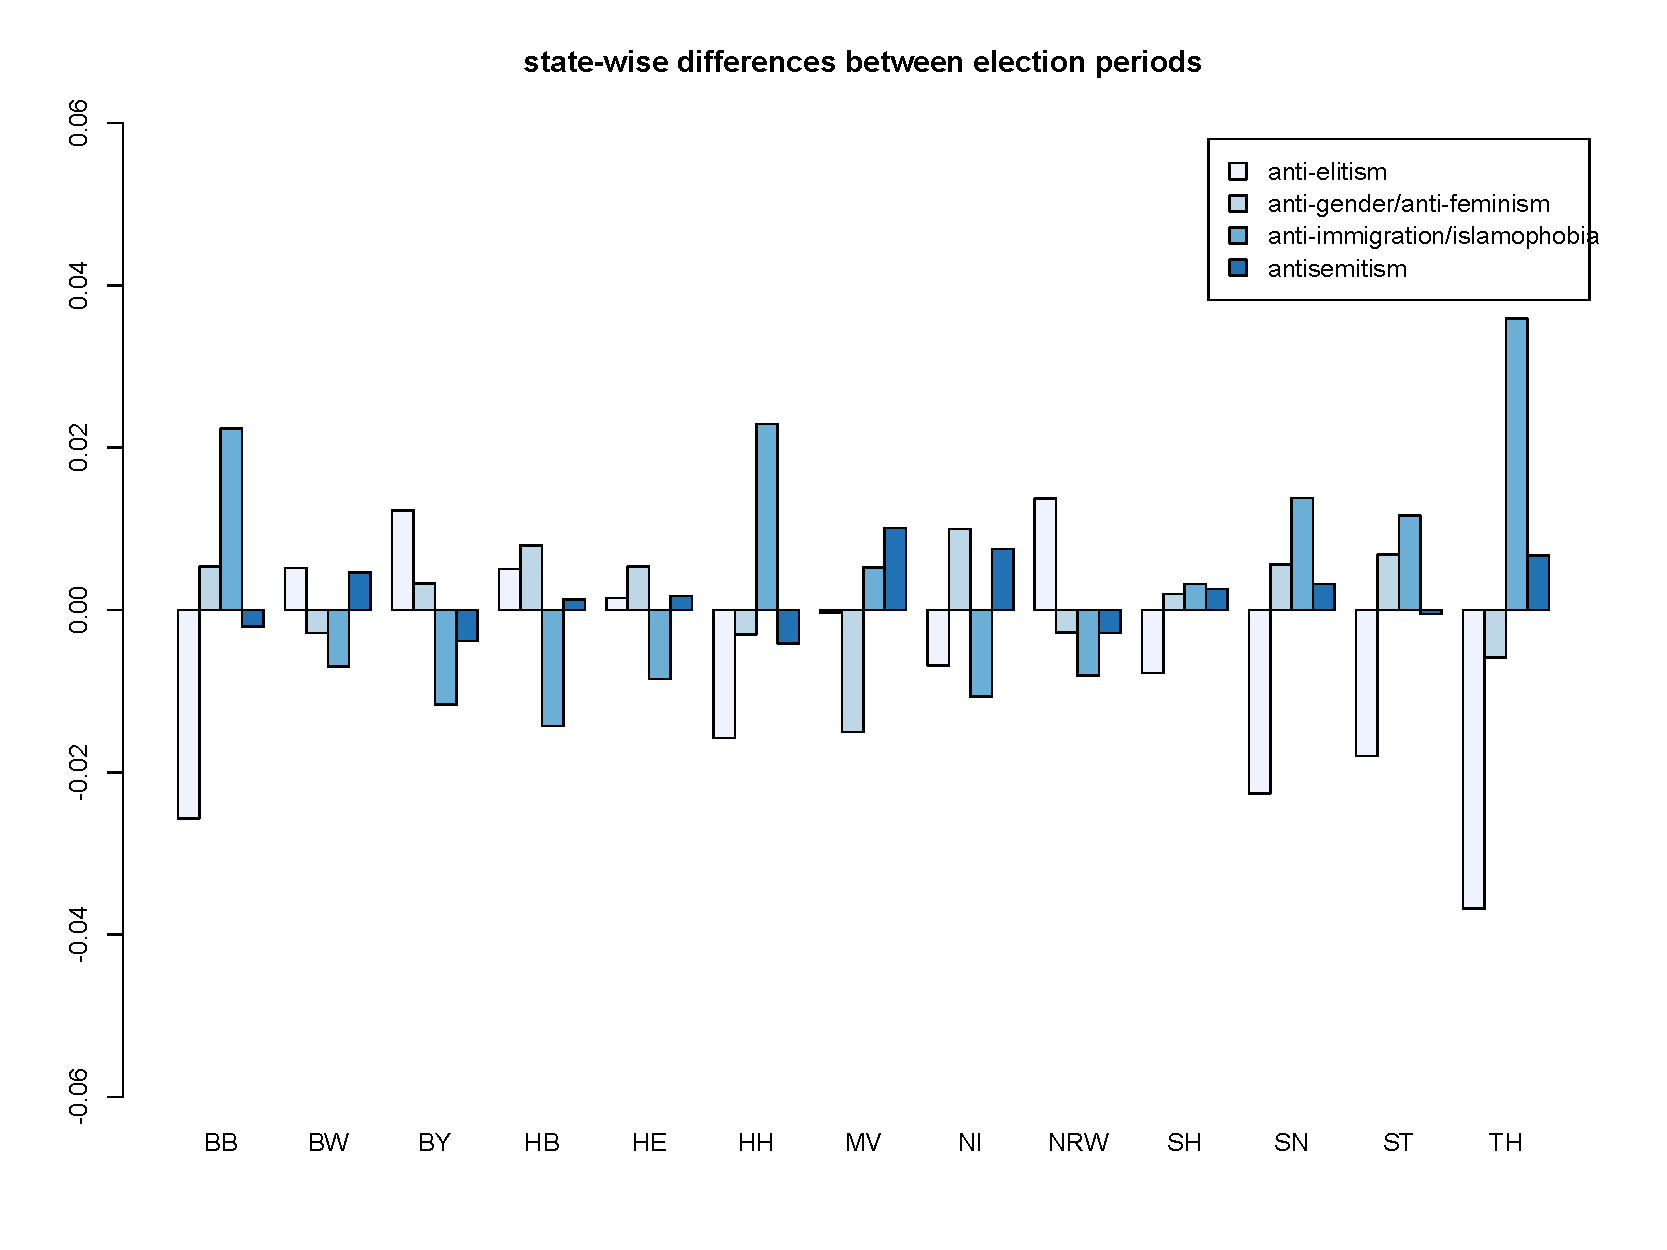
\includegraphics[width=\textwidth]{manifestos_dict_states_diffs.pdf}
    \caption{Percentage change between election periods}
    \label{fig:fig5}
\end{figure}
\begin{figure}[ht]
    \centering
    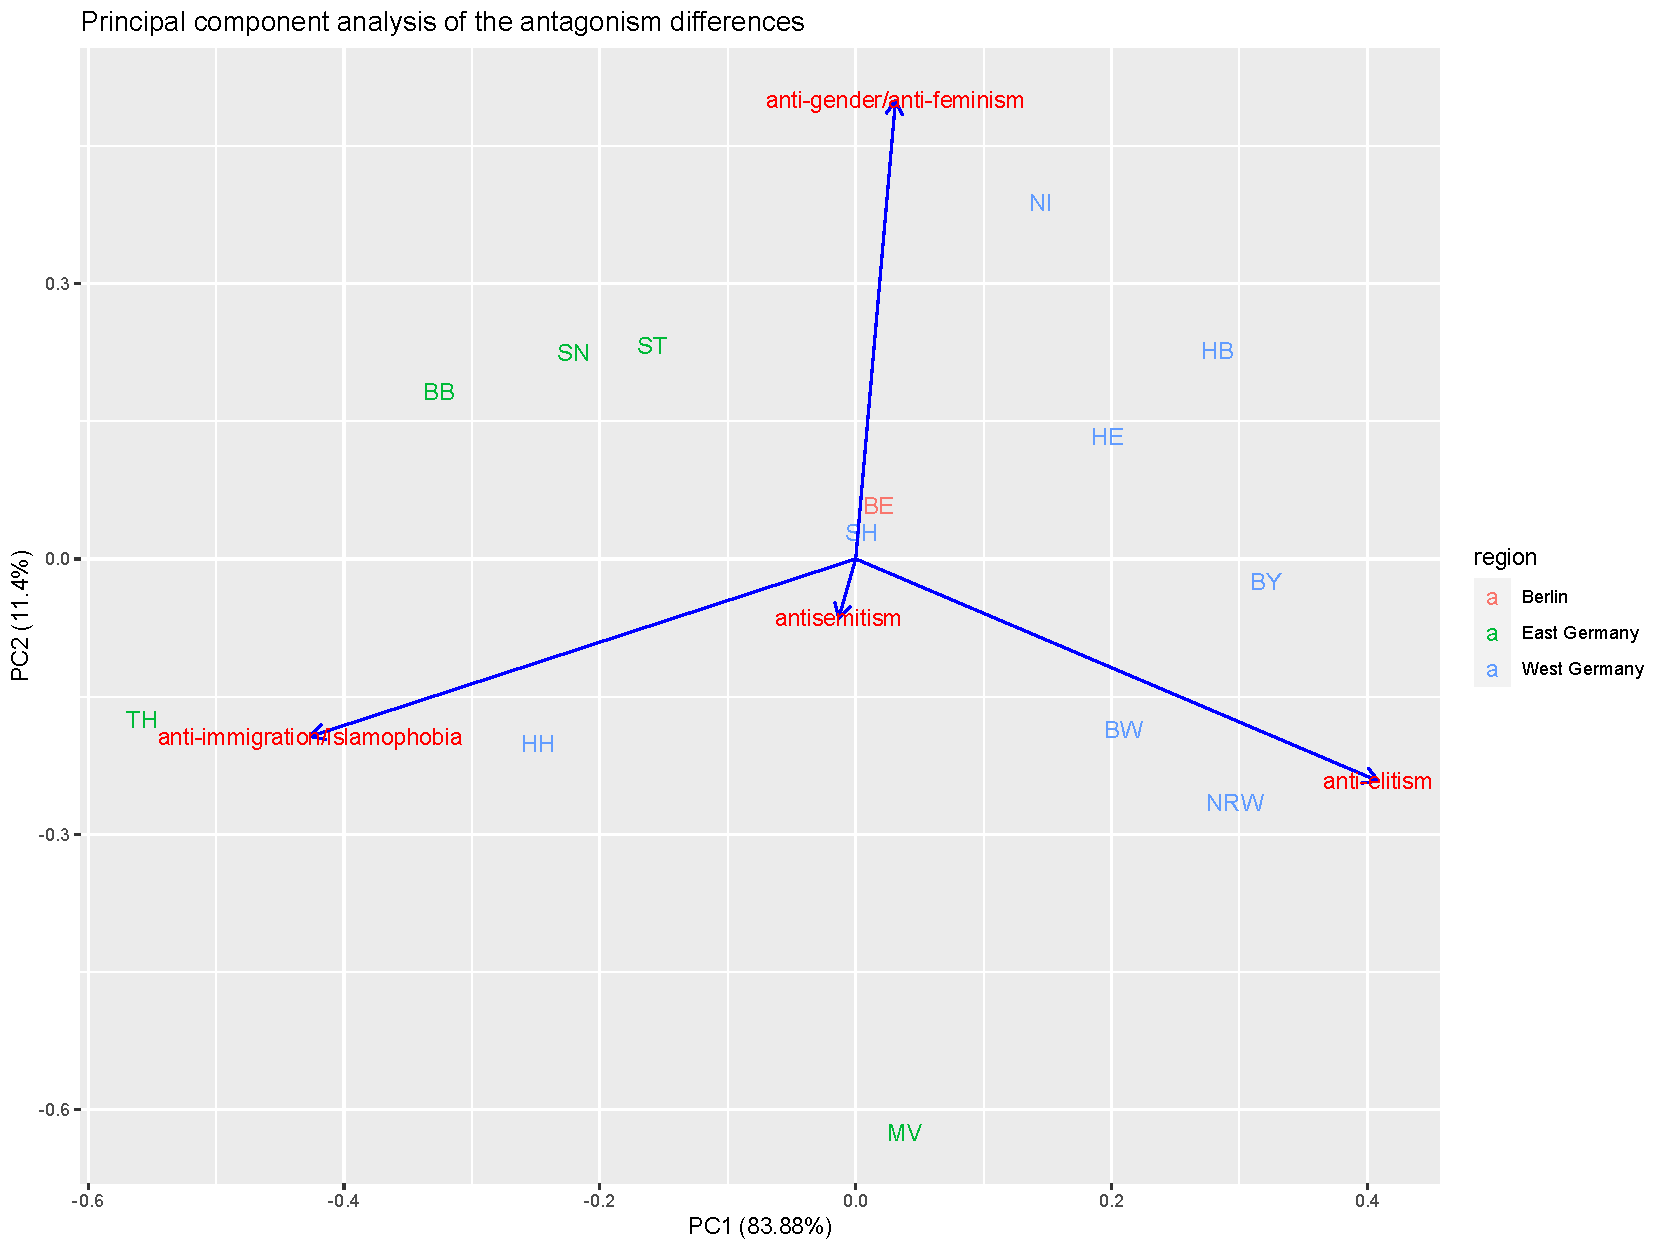
\includegraphics[width=\textwidth]{manifestos_diffs_pca.pdf}
    \caption{Pricipal component analysis}
    \label{fig:fig6}
\end{figure}
However, the resulting barplot is less intuitive for recognizing regional patterns within the ideological change. We thus aim for better visualization and apply a principal component analysis (PCA) to the 14 antagonism differences. Mathematically this is equivalent to a dimensionality reduction, i.e. we project all four-dimensional data points onto a two-dimensional subspace spanned by those two vectors that indicate the most significant direction of change.\footnote{In computational terms, the desired plane is the result of a singular value decomposition of the $14\times 4$ data matrix. The eigenvectors corresponding to the two greatest eigenvalues are used to span the plane.} In other words, the four values specifying one single difference can easily be visualized by a point in the plane (see Fig. \ref{fig:fig6}). The PCA initially tells us that the most significant change is located between the anti-immigrant and anti-elite categories. Compared to the older manifestos we truly see that the AfD party in Thuringia, Brandenburg, Saxony and Saxony-Anhalt intensified anti-immigrant enmities. Because the sole East-German exception is Mecklenburg-Vorpommern we can conclude that the AfD party in East Germany changed from anti-elitist attitudes to more racist narratives. More or less the opposite can be observed for the majority of West-German AfD associations: Here the party reinforced narratives against the democratic and economic elite. This outcome is interesting inasmuch as it shows a clear distinction between East and West Germany in terms of the party's ideological development, which was already supposed before. Another interesting observation is that the AfD party in Berlin shows almost no temporal changes, which indeed supports the argumentation of a pure East-West gradient.\par
With this in mind, we can proceed to analyze the ideological development in East and West Germany independently of each other. By doing some linear regression over time we might get more information on how the party modified its antagonistic articulation in both regions (without Berlin). For this, we consider the relative shares of one antagonism category and plot them along the election years. This approach might demonstrate how the usage of each antagonism has changed over time, in East Germany as well as in West Germany. Figure \ref{fig:fig7} at first shows the situation in West Germany with one regression model for each antagonism. As the principal component analysis already suggested, we observe an increasing linear trend for anti-elitist antagonisms whereas the anti-immigrant articulation decreases to some extent linearly. While both the red and cyan regression lines indicate a certain temporal change, the less dominant antisemitic and anti-gender language nearly remains constant over time. Furthermore, according to East Germany and figure \ref{fig:fig8}, the linear interpolation explicitly shows how the language has successively shifted to more racist and less populist narratives. Again, the fitted regression lines are well-suited to describe the development and the obtained growth rate for the anti-immigrant language is even relatively high. The usage of antisemitic and anti-gender narratives, however, is again nearly constant over time.\par
The temporal analysis of the manifestos can be summed up in saying that East-German AfD associations increasingly tend to extremist and racist positions. Their discursive construction of {\em the people} is still based on the suspicion of democratic institutions but ethnic aspects have also become relevant when it comes to the dichotomous division between {\em us} and {\em them}. In this sense, our analysis proved that the AfD party is indeed not homogeneous. Depending on the region their programmatic discourse developed differently and, thus, consists of slightly different ideological core elements - `classical' populism is the basis and xenophobia is becoming the second central core in East Germany.
\begin{figure}[ht]
    \centering
    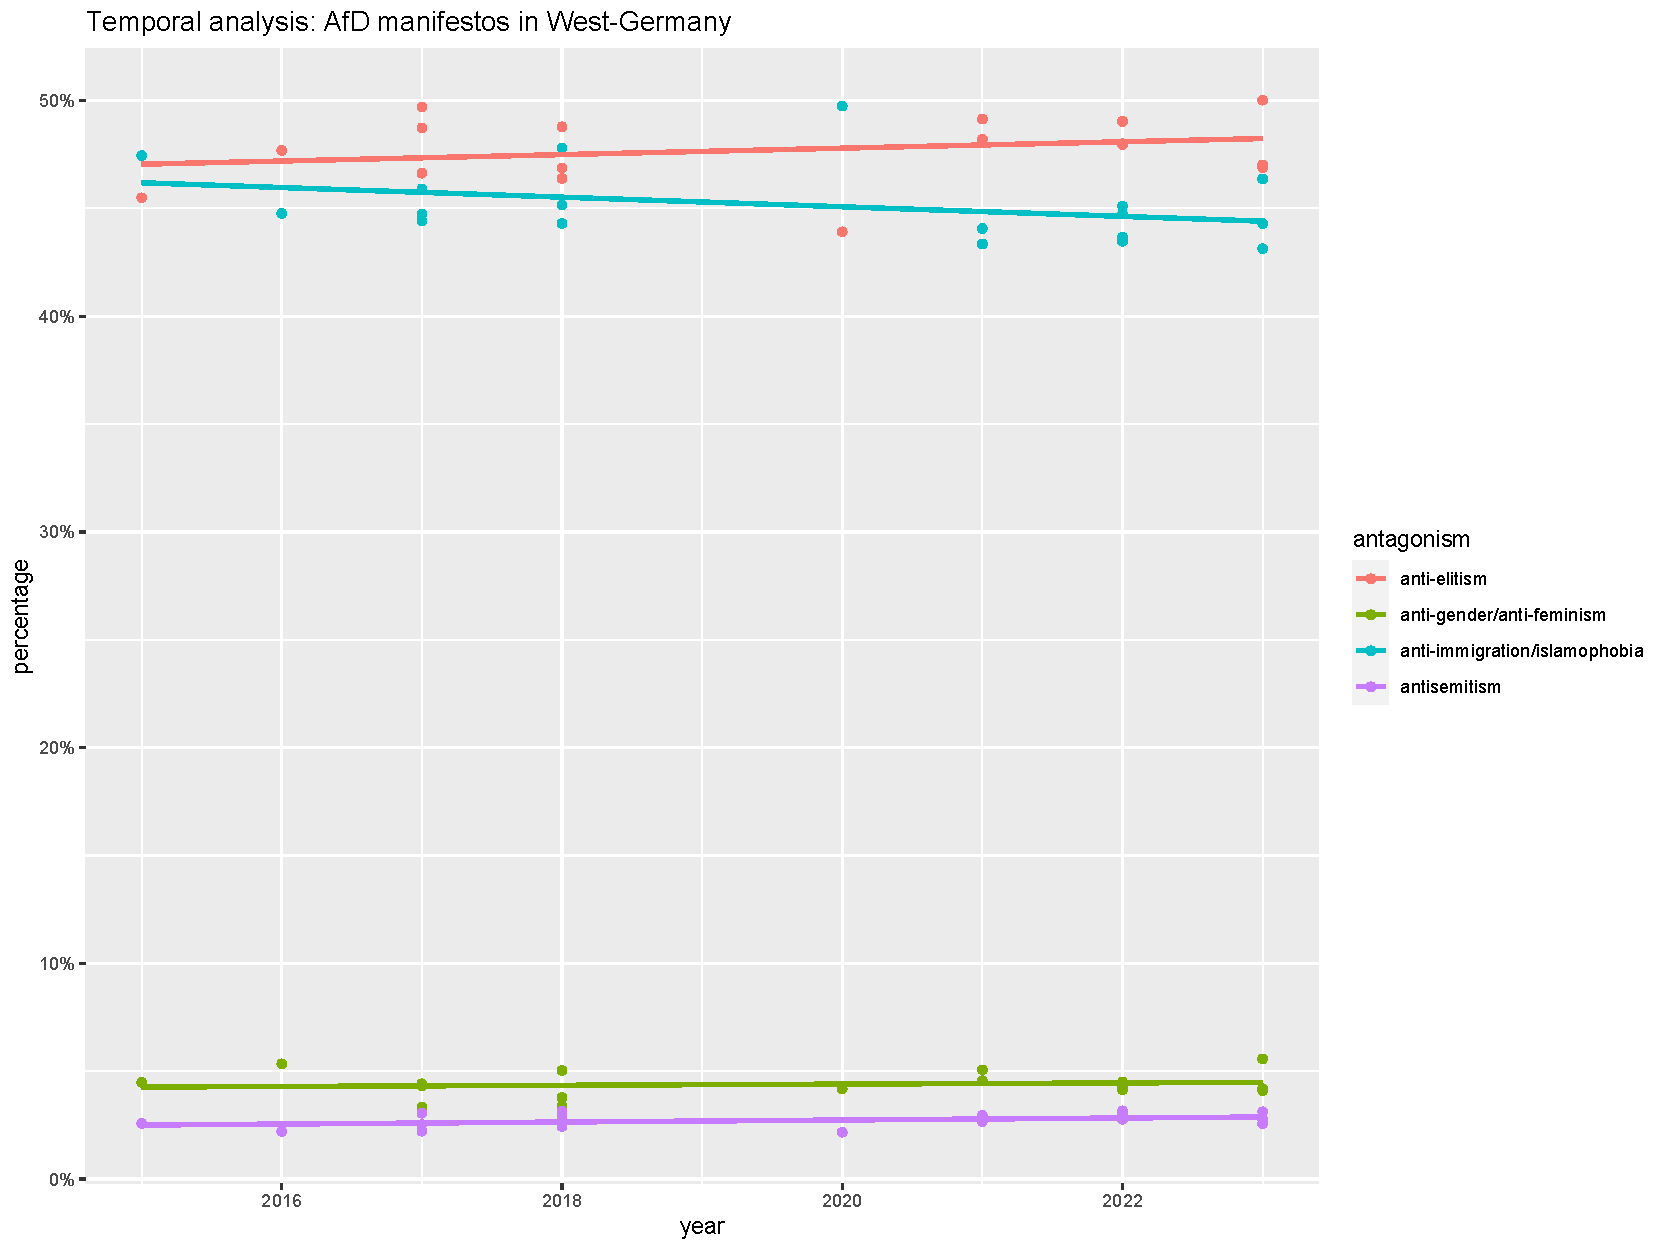
\includegraphics[width=\textwidth]{manifestos_temporal_regression_west.pdf}
    \caption{Linear regressions over time in West Germany}
    \label{fig:fig7}
\end{figure}
\begin{figure}[ht]
    \centering
    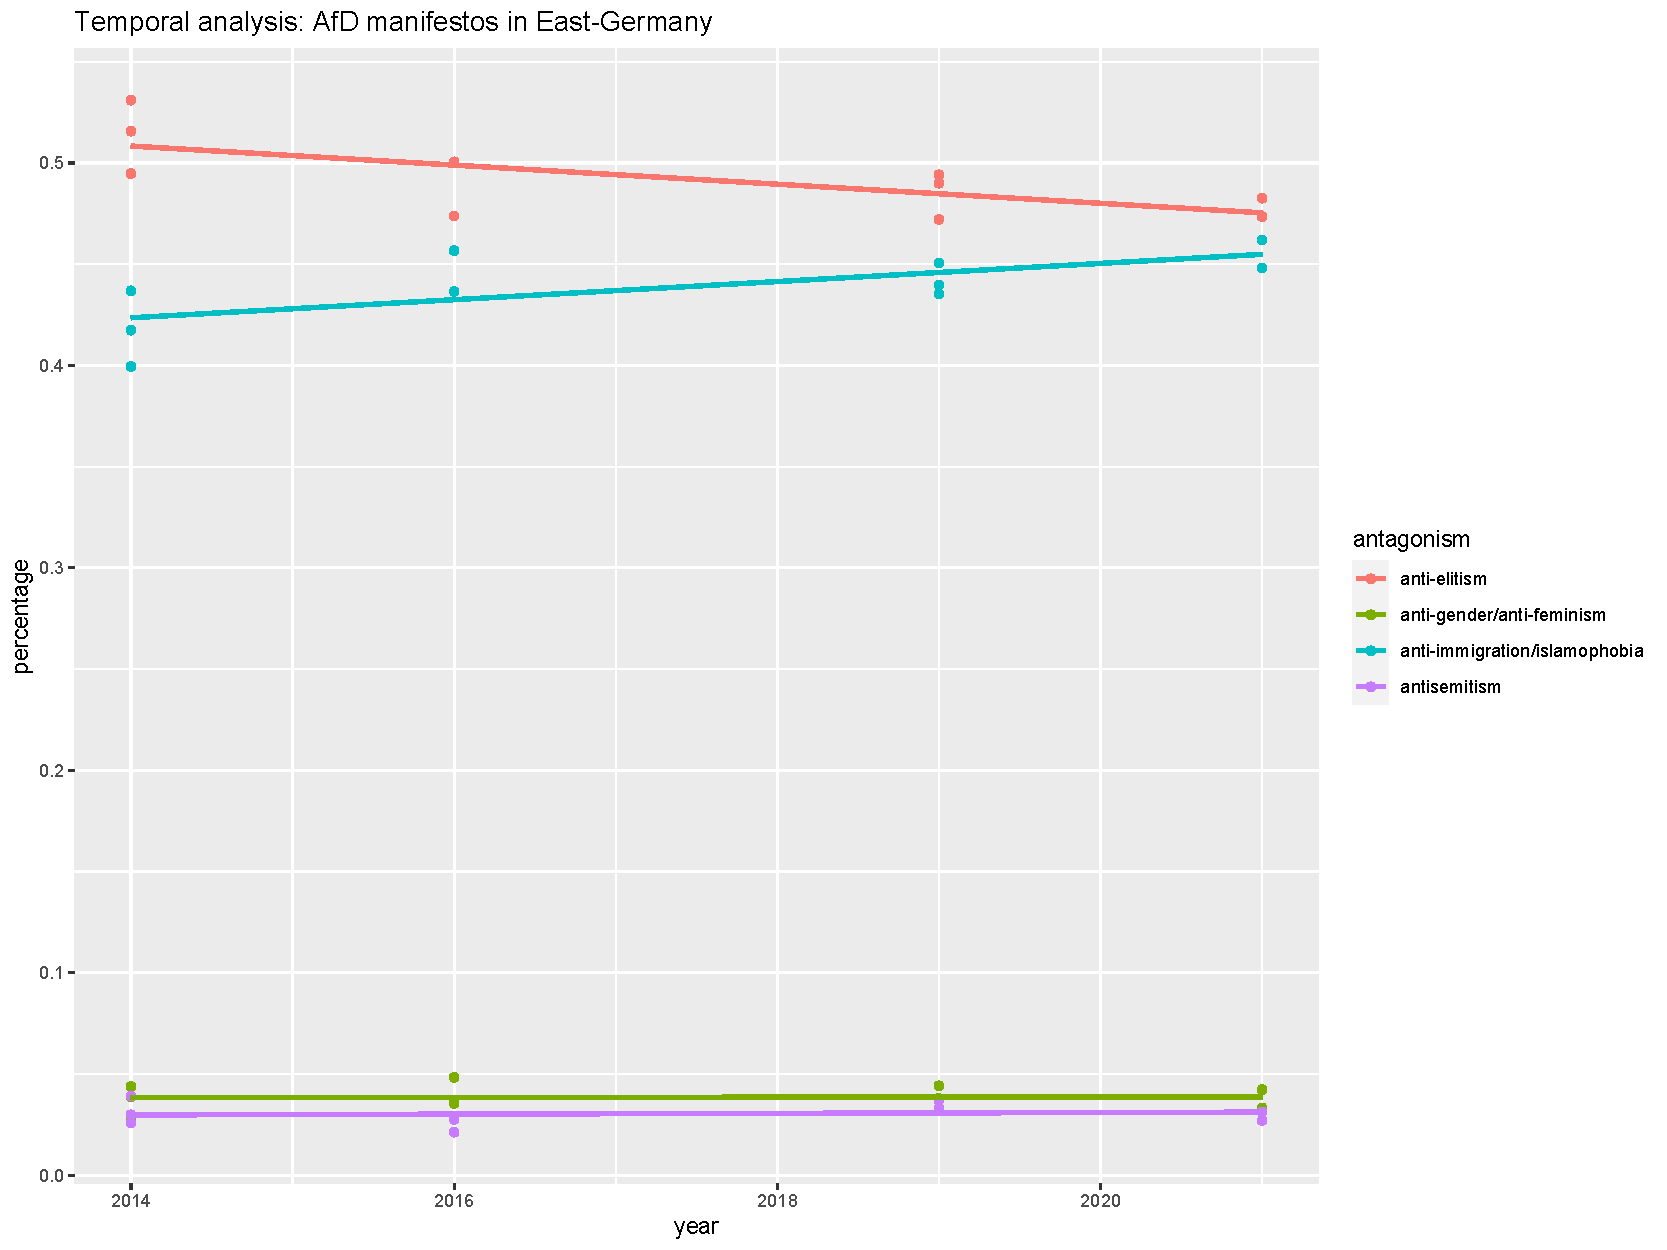
\includegraphics[width=\textwidth]{manifestos_temporal_regression_east.pdf}
    \caption{Linear regressions over time in East Germany}
    \label{fig:fig8}
\end{figure}
%%%%%
% 5 %
%%%%%
\chapter{Evaluation of the findings}
Each dictionary-based content analysis has one central bottleneck: the dictionary in itself. The methodological quality of the whole analysis depends heavily on the quality of the dictionary and its keyword lists. Thus, this chapter will evaluate all present findings by taking a renewed look at the {\em RPC-Lex}. Particularly because the {\em RPC-Lex} as a computerized generated dictionary might contain words only for statistical reasons, it is advisable to validate the provided classifications. In the following, I will elaborate on two aspects of validation that is, the classification accuracy of the dictionary and the reliability of measurements.\par
According to the classification accuracy, the question is which keywords from the dictionary are the unique classifiers related to the own corpus? Is the pre-trained dictionary anyway able to reasonably classify the corpus? In our case, the answer is yes (not least because the authors have extensively tested the dictionary). Especially the classification of anti-elitist and anti-immigrant content seems to be satisfying. Figure \ref{fig:fig9} lists a selection of unique classifiers and one can see that both mentioned categories have the most. However, the classification of antisemitic antagonisms is only based on a few keywords and, thus, must be evaluated critically. Here not only the small number of words is the problem but also the insignificance of the available classifiers (e.g. ``zeigt'', ``beste''). Consequently, the classification of antisemitic language is most likely less accurate than for the other antagonisms.\par
\begin{figure}
    \centering
    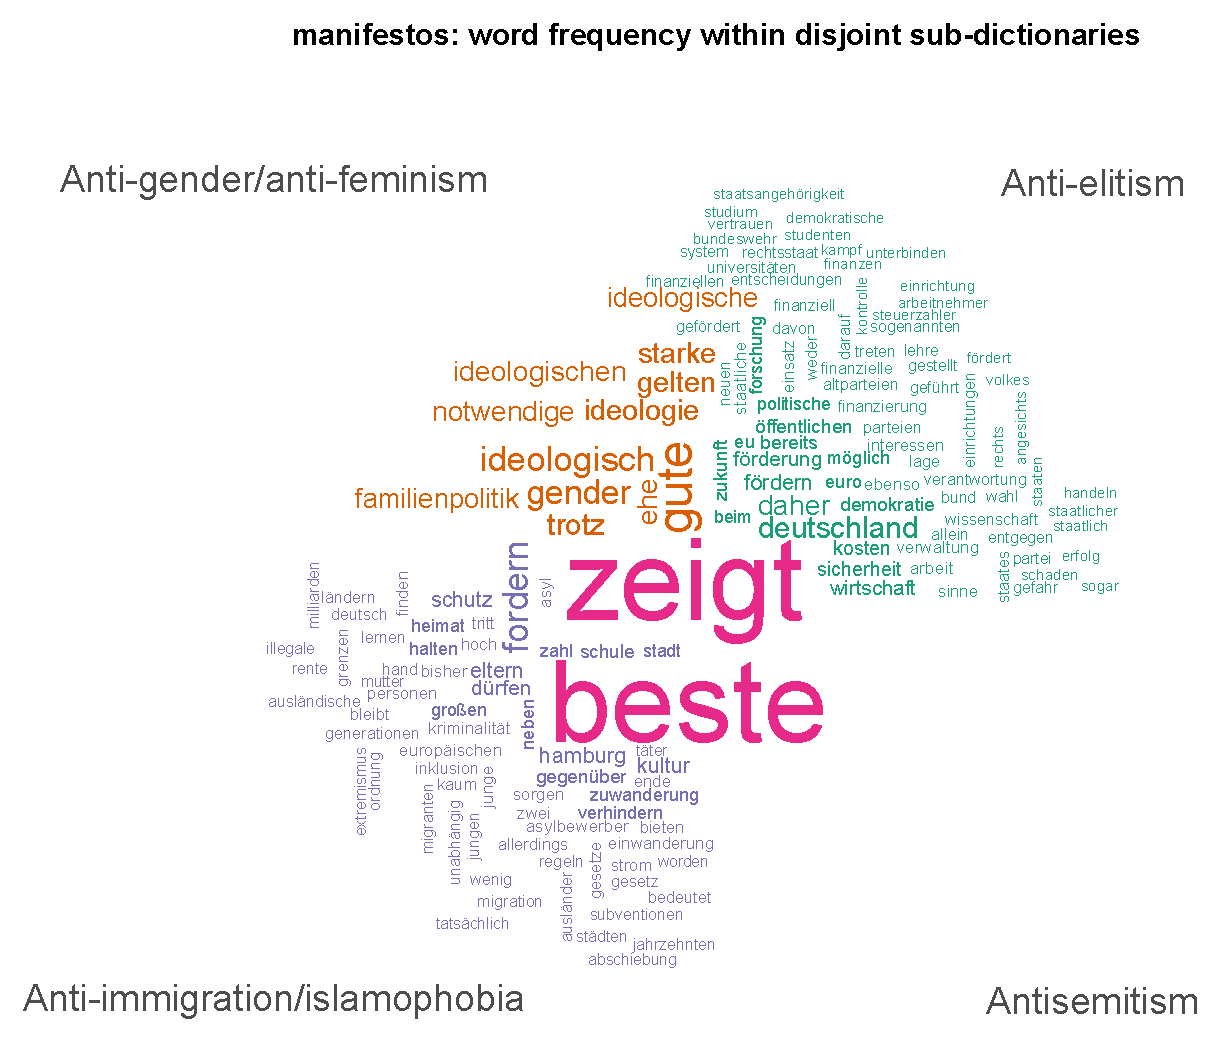
\includegraphics[width=0.75\textwidth]{manifestos_wordcloud_disjoint_subdicts-crop.pdf}
    \caption{Unique classifiers for all antagonism categories}
    \label{fig:fig9}
\end{figure}
The second aspect refers to the intensified anti-immigrant discourse in East Germany and the intensified anti-elite discourse in West Germany, respectively. To validate these findings we want to figure out which keywords from the {\em RPC-Lex} have caused the growth between the two election periods. This implies that we need to determine all those keywords being predominantly present in the last manifestos but not in the manifestos before. The resulting word clouds can be found in Fig. \ref{fig:fig10} and Fig. \ref{fig:fig11}. As one can see, the increasing number of anti-elitist antagonisms within West-German AfD manifestos can be traced back to keywords indicating a clear nationalist and populist position (e.g. ``unserer'', ``unser'', ``Bürger'', ``Deutschland'', ``EU''). In this sense the increase within the anti-elitist language is plausible. For the anti-immigrant discourse in East Germany, however, the rising number of racist terms is difficult to validate. The growth rate is mainly caused by keywords like ``Land'', ``Schutz'', ``Heimat'', ``Schulen'', ``Geld'' which do not directly relate to a racist discourse. Such terms can admittedly be used in racist statements but, as single signifiers, they are rather inappropriate for validating the results. At this point, more effort is necessary to be able to emphasize the racist tendencies in East-German AfD manifestos. 
\begin{figure}
    \centering
    \begin{minipage}{.5\textwidth}
        \centering
        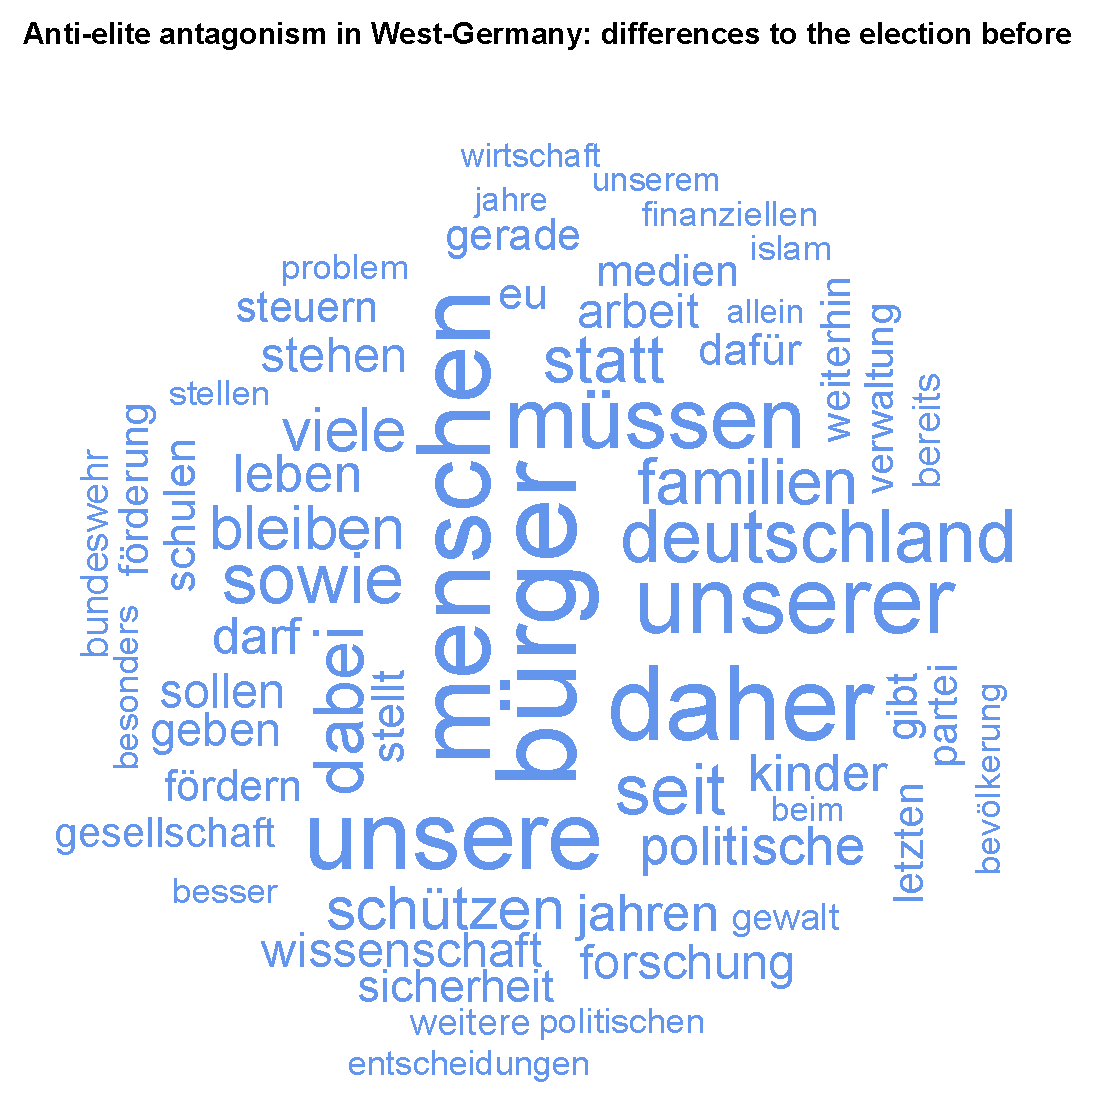
\includegraphics[width=0.85\textwidth]{manifestos_wordcloud_diffs_west-crop.pdf}
        \caption{Rising anti-elite terms}
        \label{fig:fig10}
    \end{minipage}%
    \begin{minipage}{.5\textwidth}
        \centering
        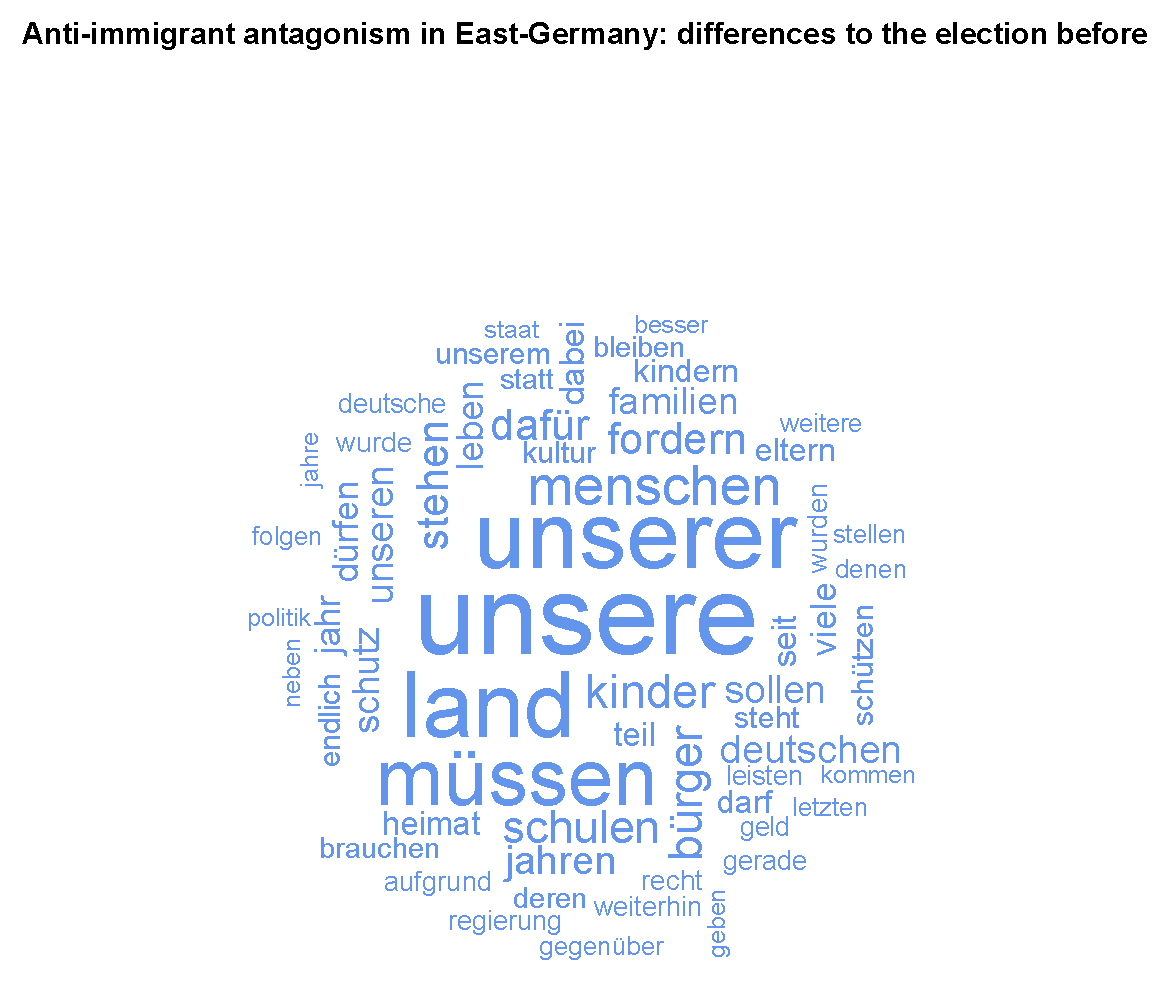
\includegraphics[width=\textwidth]{manifestos_wordcloud_diffs_east-crop.pdf}
        \caption{Rising anti-immigration terms}
        \label{fig:fig11}
    \end{minipage}
\end{figure}
%%%%%
% 6 %
%%%%%
\chapter{Conclusion and final comments}

\bibliography{refs}

\end{document}